\documentclass[]{article}
\usepackage{lmodern}
\usepackage{amssymb,amsmath}
\usepackage{ifxetex,ifluatex}
\usepackage{fixltx2e} % provides \textsubscript
\ifnum 0\ifxetex 1\fi\ifluatex 1\fi=0 % if pdftex
  \usepackage[T1]{fontenc}
  \usepackage[utf8]{inputenc}
\else % if luatex or xelatex
  \ifxetex
    \usepackage{mathspec}
  \else
    \usepackage{fontspec}
  \fi
  \defaultfontfeatures{Ligatures=TeX,Scale=MatchLowercase}
\fi
% use upquote if available, for straight quotes in verbatim environments
\IfFileExists{upquote.sty}{\usepackage{upquote}}{}
% use microtype if available
\IfFileExists{microtype.sty}{%
\usepackage{microtype}
\UseMicrotypeSet[protrusion]{basicmath} % disable protrusion for tt fonts
}{}
\usepackage[margin=0.6in]{geometry}
\usepackage{hyperref}
\hypersetup{unicode=true,
            pdftitle={Large-Sample Normal Approximation to the Posterior},
            pdfborder={0 0 0},
            breaklinks=true}
\urlstyle{same}  % don't use monospace font for urls
\usepackage{graphicx,grffile}
\makeatletter
\def\maxwidth{\ifdim\Gin@nat@width>\linewidth\linewidth\else\Gin@nat@width\fi}
\def\maxheight{\ifdim\Gin@nat@height>\textheight\textheight\else\Gin@nat@height\fi}
\makeatother
% Scale images if necessary, so that they will not overflow the page
% margins by default, and it is still possible to overwrite the defaults
% using explicit options in \includegraphics[width, height, ...]{}
\setkeys{Gin}{width=\maxwidth,height=\maxheight,keepaspectratio}
\IfFileExists{parskip.sty}{%
\usepackage{parskip}
}{% else
\setlength{\parindent}{0pt}
\setlength{\parskip}{6pt plus 2pt minus 1pt}
}
\setlength{\emergencystretch}{3em}  % prevent overfull lines
\providecommand{\tightlist}{%
  \setlength{\itemsep}{0pt}\setlength{\parskip}{0pt}}
\setcounter{secnumdepth}{0}
% Redefines (sub)paragraphs to behave more like sections
\ifx\paragraph\undefined\else
\let\oldparagraph\paragraph
\renewcommand{\paragraph}[1]{\oldparagraph{#1}\mbox{}}
\fi
\ifx\subparagraph\undefined\else
\let\oldsubparagraph\subparagraph
\renewcommand{\subparagraph}[1]{\oldsubparagraph{#1}\mbox{}}
\fi

%%% Use protect on footnotes to avoid problems with footnotes in titles
\let\rmarkdownfootnote\footnote%
\def\footnote{\protect\rmarkdownfootnote}

%%% Change title format to be more compact
\usepackage{titling}

% Create subtitle command for use in maketitle
\newcommand{\subtitle}[1]{
  \posttitle{
    \begin{center}\large#1\end{center}
    }
}

\setlength{\droptitle}{-2em}

  \title{Large-Sample Normal Approximation to the Posterior}
    \pretitle{\vspace{\droptitle}\centering\huge}
  \posttitle{\par}
    \author{}
    \preauthor{}\postauthor{}
    \date{}
    \predate{}\postdate{}
  
\usepackage{multicol}

\begin{document}
\maketitle

\def\simiid{\stackrel{{\mbox{\text{\tiny i.i.d.}}}}{\sim}}

\section{Poisson Model}\label{poisson-model}

\begin{itemize}
\tightlist
\item
  Observe \(X_1, \ldots, X_n\); \(X_i\) is the number of seedlings in
  quadrat number \(i\).
\item
  Data Model:
  \(X_i | \Lambda = \lambda \simiid \text{Poisson}(\lambda)\)
\item
  Suppose we use a Gamma prior for \(\Lambda\)

  \begin{itemize}
  \tightlist
  \item
    Example: \(\Lambda \sim \text{Gamma}(1, 0.01)\) is fairly
    non-informative
  \end{itemize}
\item
  Decomposing the log-posterior pdf into contributions from prior and
  likelihood
\end{itemize}

\(\log\{f_{\Theta | X_1, \ldots, X_n}\} = \log\{ c \cdot f_{\Theta}(\theta) \cdot \prod_{i=1}^n f_{X_i|\Theta}(x_i | \theta) \} = \log(c) + \log\{f_{\Theta}(\theta)\} + \sum_{i=1}^n \log\{ f_{X_i|\Theta}(x_i | \theta) \}\)

\subsection{\texorpdfstring{Simulation:
\(\lambda = 10\)}{Simulation: \textbackslash{}lambda = 10}}\label{simulation-lambda-10}

\paragraph{n = 1}\label{n-1}

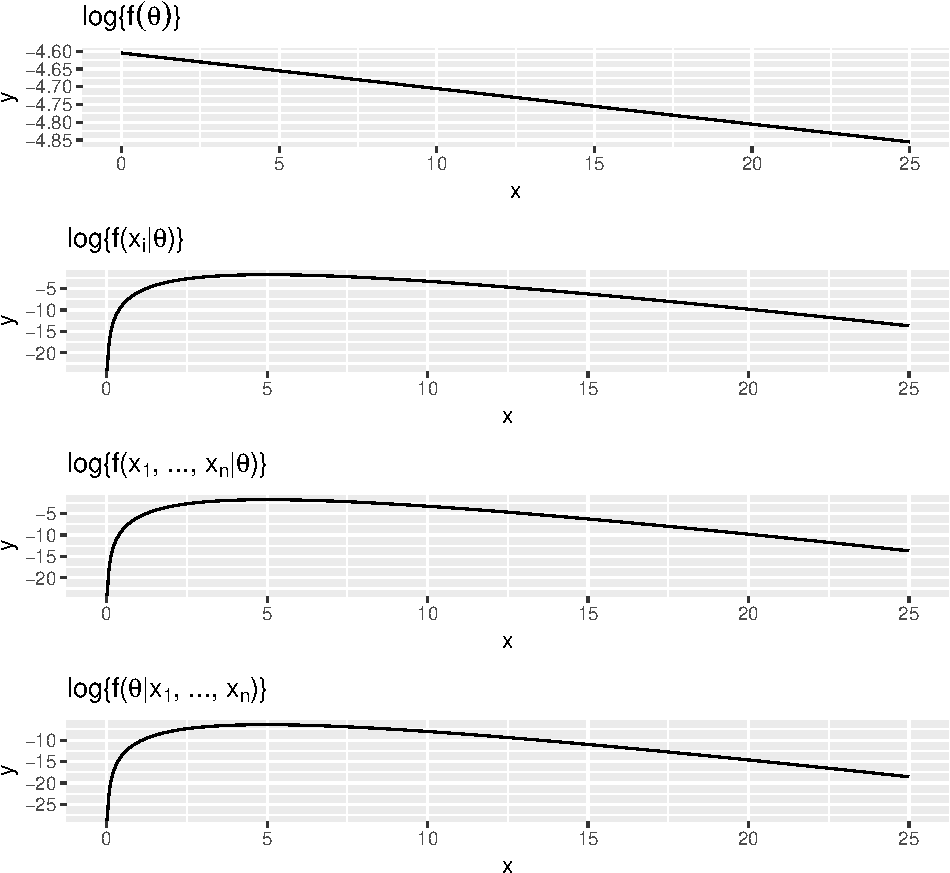
\includegraphics{20190306_log_posterior_contributions_files/figure-latex/unnamed-chunk-2-1.pdf}

\newpage

\paragraph{n = 10}\label{n-10}

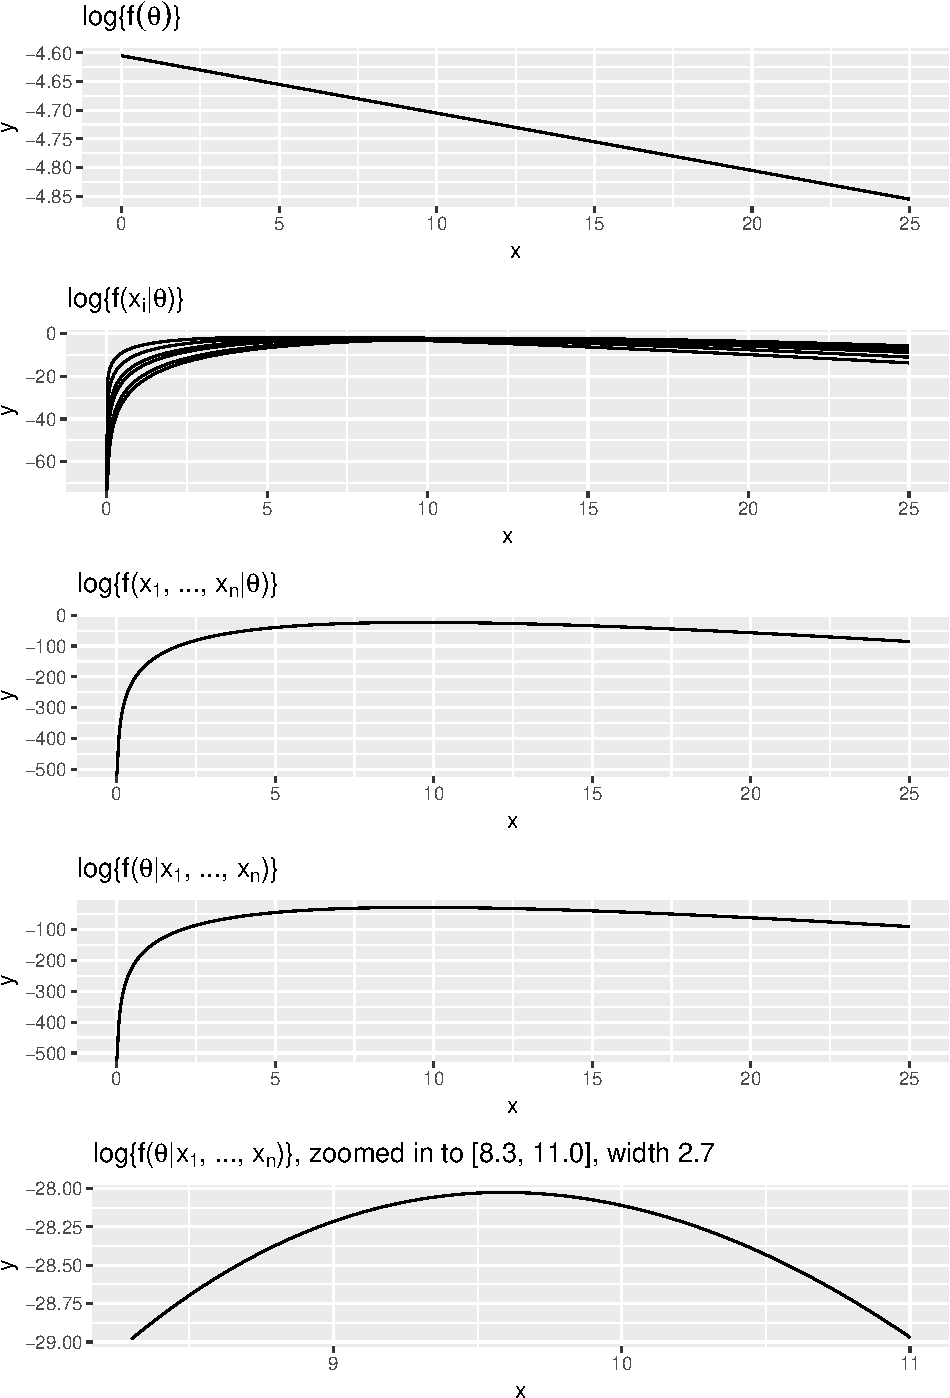
\includegraphics{20190306_log_posterior_contributions_files/figure-latex/unnamed-chunk-4-1.pdf}
\newpage

\paragraph{n = 100}\label{n-100}

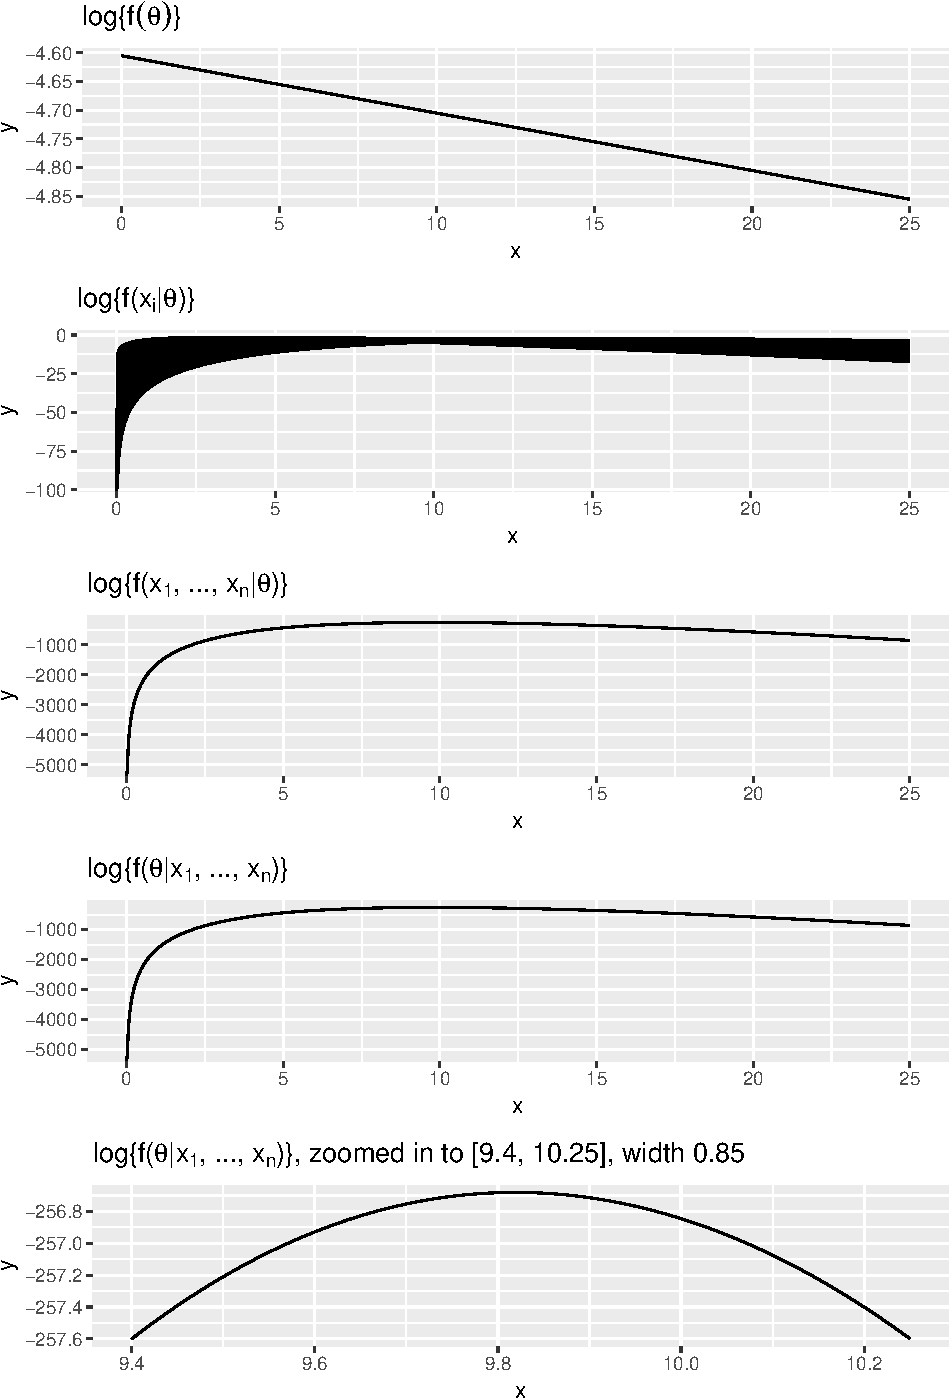
\includegraphics{20190306_log_posterior_contributions_files/figure-latex/unnamed-chunk-6-1.pdf}

\newpage

\paragraph{n = 1000}\label{n-1000}

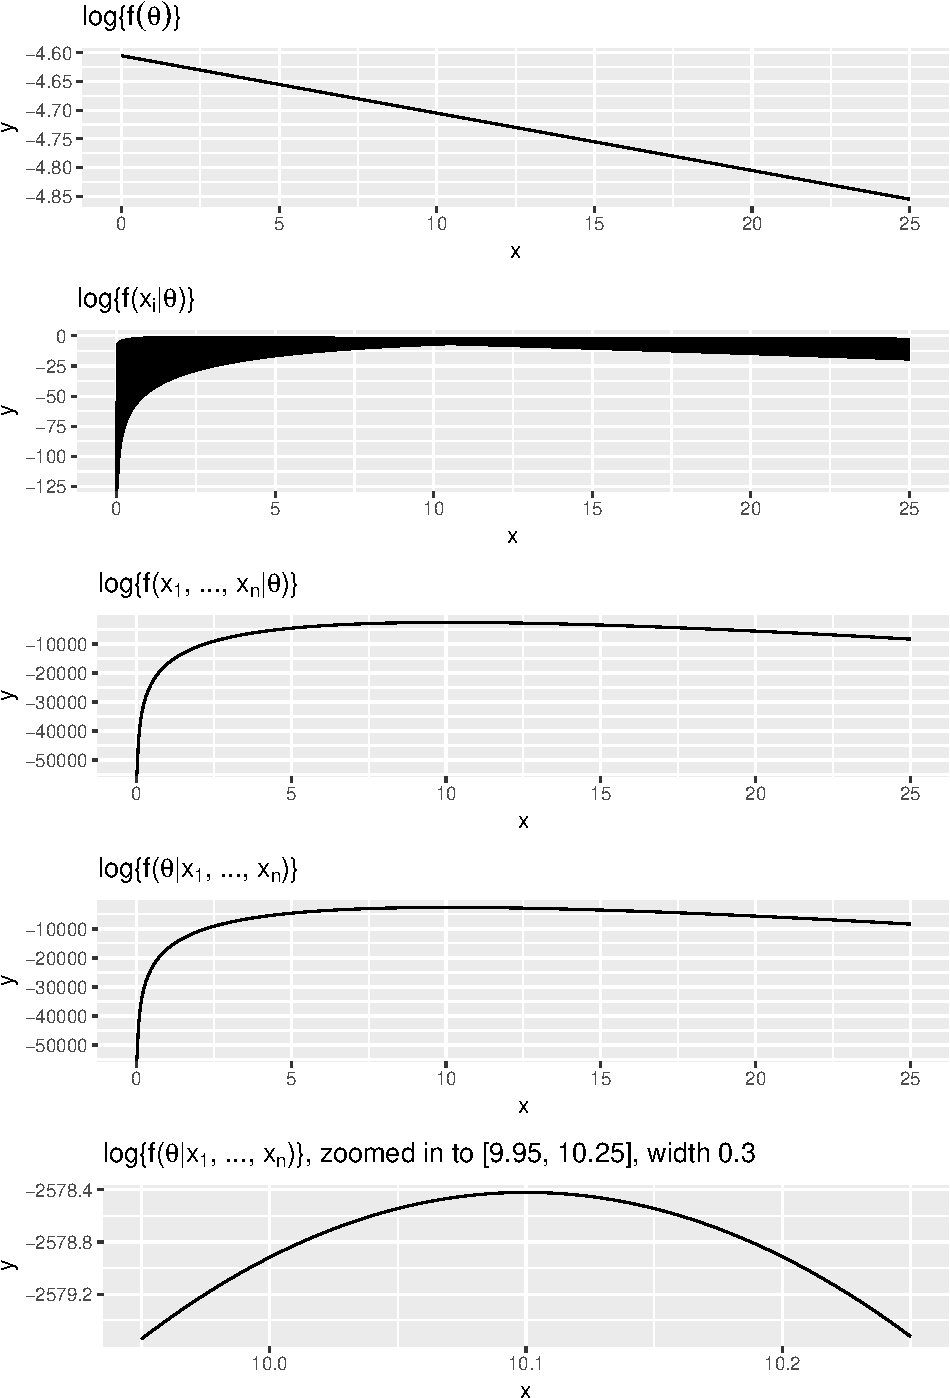
\includegraphics{20190306_log_posterior_contributions_files/figure-latex/unnamed-chunk-8-1.pdf}


\end{document}
